\documentclass{aiaa-tc}% insert '[draft]' option to show overfull boxes

\usepackage{graphicx}
\usepackage{amsmath}
\usepackage{calc}%allows for scaling figures with integer division/multiplication of existing lengths
\usepackage{wrapfig}
\usepackage{lipsum}
\usepackage[hidelinks]{hyperref}
%\usepackage{hyperref}
%\usepackage{biblatex}

\title{Design and Manufacture of an Open-Hardware 
 	University Rocket Airframe using Carbon Fiber}

\author{
Joseph Shields, Leslie Elwood, Erik Nelson, and Jacob East%, Brandon Bonner
	\thanks{Portland State University, Portland, OR 97201}
 }
% Data used by 'handcarry' option if invoked
\AIAApapernumber{2016}
\AIAAconference{Conference Name, Date, and Location}
\AIAAcopyright{\AIAAcopyrightD{2016}}
\bibliographystyle{aiaa}
 
% Define commands to assure consistent treatment throughout document
\newcommand{\eqnref}[1]{(\ref{#1})}
\newcommand{\class}[1]{\texttt{#1}}
\newcommand{\package}[1]{\texttt{#1}}
\newcommand{\file}[1]{\texttt{#1}}
\newcommand{\BibTeX}{\textsc{Bib}\TeX}
\newcommand{\cots}{commercial off-the-shelf}
\newcommand{\weightReduction}{80\%}
\newcommand{\strengthIncrease}{??\%}

\begin{document}
\maketitle
% Hello

\begin{abstract}
The amateur and university rocketry communities are rapidly reaching higher altitudes with more sophisticated rockets. However, most groups are still using heavy airframes made of metal or fiberglass. Commercial off-the-shelf airframes are either too expensive for low-budget university groups or too small to use as a platform for high altitude experiments. 
A capstone team of mechanical engineering seniors at Portland State University has developed a low-weight, modular carbon fiber airframe as an open-hardware technology for university rocketry. 
This project continues the work of a 2014 capstone team, who developed a carbon fiber layup process with promising results. 
This will enable low-budget groups like the Portland State Aerospace Society to explore high altitude science and compete in the university space race.  \end{abstract}
\section*{Nomenclature}
\begin{itemize}
	\item CFD, Computational Fluid Dynamics
	\item PSAS, Portland State Aerospace Society
	\item LV2, Launch Vehicle 2
	\item LV3, Launch Vehicle 3
	\item HPR, High Power Rocketry
\end{itemize}


\section{Introduction}
%REMEMBER TO SPECIFY ALL ACRONYMS/INITIALISMS!
The Portland State Aerospace Society (PSAS) is an interdisciplinary group of engineering students and alumni of Portland State University (PSU) with the long term goal of putting a cubesat into orbit with their own rocket. 
% info about cubesat market growth: http://www.spaceref.com/news/viewpr.html?pid=44940 
Their current airframe, named Launch Vehicle 2 (LV2), has served for over 12 years, representing 10 of the group's 13 launches, and hosted experiments ranging from custom patch antennas and long range WiFi technology to GPS navigation and a cold gas reaction control system (figure \ref{fig:L-12}). The LV2 platform is mostly constructed of aluminum with a fiberglass shell, with many of the parts having been fabricated in home garages. This makes for a robust but heavy design. Additionally, this airframe is built with a 4.5 inch inner diameter which PSAS's experiments have outgrown. 

\begin{wrapfigure}{R}{\linewidth/3}
\centering
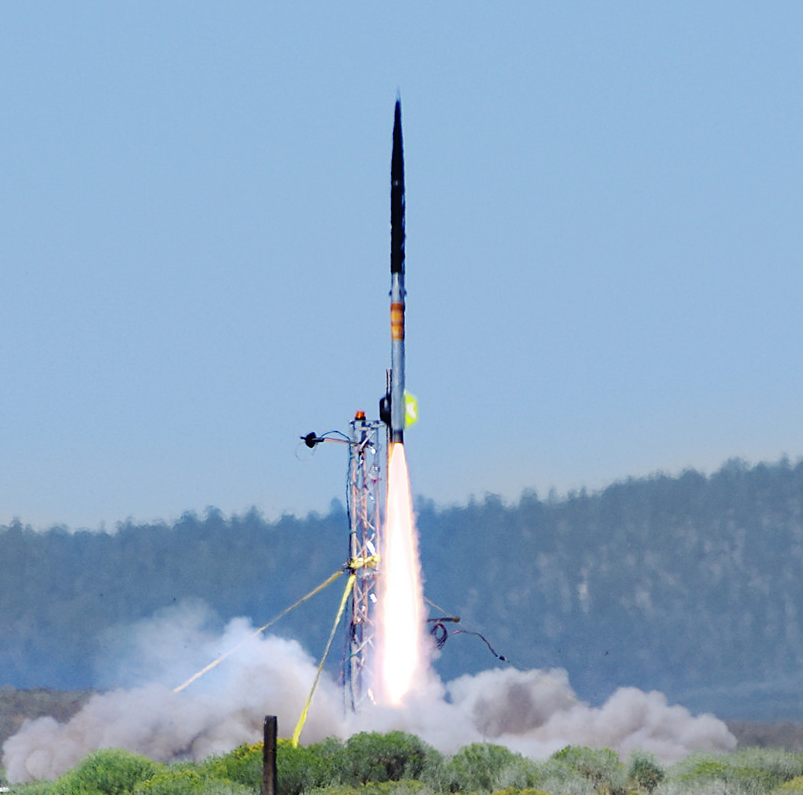
\includegraphics[width=\linewidth]{../img/L12-cropped.png}
\caption{PSAS's LV2 rocket lifting off for the group's $13^\text{th}$launch. The custom cylindrical patch antenna can be seen as a brown band around the middle of the rocket.}
\label{fig:L-12}
\end{wrapfigure}

The new airframe being designed, named Launch Vehicle 3 (LV3), aims to address these issues. The LV3 platform uses a 6 inch inner diameter, modules composed of carbon fiber and thin aluminum coupling rings, a carbon fiber nose cone, and a carbon fiber fin section. All of the airframe components connect via standardized rings, to accommodate future experimental modules and flight configurations.
The cylindrical LV3 airframe modules outperform the old design with an \weightReduction{} reduction in weight.
% Do we know what the increase in strength is? Also, can we confirm the weight reduction?

\subsection{Basic Design}
%----------insert a diagram and/or picture of the sandwich design----------
The majority of the LV3 airframe uses a sandwich shell composed of CF faces surrounding an aramid honeycomb core. This provides a rigid structure while minimizing weight. 
Single sheets of carbon fiber are rigid when subjected to in-plane loading, but very flexible under out-of-plane loading. Similarly, the core is flexible under in-plane loading, but rigid under out-of-plane compression. 
When laminated together, these form a plate which is rigid in all loading conditions. The core material separates the rigid CF faces, greatly increasing the second moment of inertia of the plate. There is much more to the theory of sandwich plates and beams, but that is outside the scope of this paper. 

The body of the airframe is composed of modular cylindrical sections using this sandwich design with aluminum coupling rings co-molded to each end.
Each module can hold avionics, experiments, or other equipment with six tapped holes around the inside of the female coupling ring. 
For the radio module, FG takes the place of the CF to allow radio transparency.

The fins use the same sandwich design, with an aluminum frame defining their planform. The center of the frame is filled with core material, and the whole surface is covered in carbon fiber. 
The leading and trailing edges of the fins are made of machined phenolic resin, co-bonded with the frame and CF faces. 
The fins are fins are attached to a module with epoxy fillets, using chopped CF as a filler, and "tip-to-tip" CF sheets running from the tip of one fin accross the module to the tip of the other fin.

The nose cone uses the same coupling ring system as the modules. It is a von K\'arm\'an ogive formed from two molded CF shells. 
Unlike the rest of the airframe, the nose cone uses a thin shell of two CF sheets, rather than a sandwich design (see section \ref{sec:noseCone} for details). 
The tip of the nose cone is machined out of aluminum and is removed when assembling the recovery system inside the nose cone. 

\subsection{Significance}
Many amateur and university rocketry groups use composite airframes. However, these designs use many layers of fabric, with low fiber volume fractions.
While easy and durable, this does not fully take advantage of their materials. The LV3 design achives a much higher specific strength and rigidity, enabling greater altitudes with a given motor. 

This design also occupies an uncommon regime for sandwich shell designs. Most such designs use sandwich shells in large, low curvature parts, whereas the LV3 modules have a relatively small size and high curvature.

This is also the only fully open-hardware rocket airframe in the HPR level 3 range. All of the documentation, design, and testing information if freely available on PSAS's Github page \cite{LV3repo}.
%----------need to make extra-sure there aren't any other open-hardware airframes out there----------

\section{Software}
\subsection{OpenRocket}
For the early design of amateur and university-scale rockets, \href{http://openrocket.sourceforge.net/}{OpenRocket} is very useful. 
It is an open-source Java application which simulates a rocket's flight. It provides a convenient interface for configuring the rocket, selecting commercial or custom parts, viewing the predictions, and performing some basic optimization. 

Using OpenRocket to guide the initial design allowed for rapid iteration of the fin geometry and the placement of non-airframe components. 

\subsection{OpenFOAM}
OpenFOAM is another open-source application. It provides a common interface for a wide range of CFD solvers.
Although it requires more up-front effort, it allows a more detailed perspective on what features of an airframe's geometry are the most critical. 
CFD analysis is probably not necessary for most amateur and university level airframe design, but this provides a good option for groups that can't afford a licence for a commercial CFD suite. 

OpenFoam was used to asses the heating at the tip of the nose, to determine if the epoxy matrix of the carbon fiber would degrade over repeated flights.


\section{Materials}

\subsection{Acquisition}

\section{Cylindrical Modules}

\subsection{Destructive Testing}

\section{Nose Cone}\label{sec:noseCone}
To make the nose cone would take significant research into materials and ingenuity. The pre-impregnated carbon fiber material donated to us is a material with a 350 degree Fahrenheit cure cycle. Thus every element used henceforth must survive the same temperature. The initial manufacturing process involved a mandrel and the same procedure as the cylindrical modules. Machine Sciences agreed to donate the material and machine time to create this for PSAS however, lead time prevented them from delivering this to us in the time frame necessary for launch. 

After much consideration, it was decided that the next best method for creating the nose cone would be to use a mold. A 1 inch thick, high temp, 18 pound density machinable foam (FR 4718) was purchased from General Plastics and stacked to create a 4 inch thickness. ACP high-temperature resin epoxy is mixed with a 3.2:10 ratio which was used to mix this resin before application and then ran through a heat cycle to cure. Next, the foam block was transported to ESCO to be run through a CNC Mill and returned. 

The mold experience mild delamination during milling and needed extra resin to hold together. Understanding that the machinable foam is porous and would likely absorb any fluid adhesive created by the high temperature environment, and thus deform the foam blocks, it was decided that the surface of the mold would be coated in the ACP resin and run through another heat cycle. As a secondary measure to ensure the carbon fiber and adhesives would release from the mold, three layers of Fibre Glast non-silicone high temperature paste wax is applied to the surface of the mold. Once the wax set, a generous layer of Fibre Glast PVA release film was then painted to the surface. 

Using a template, carbon fiber material is cut to fit into the mold. Because of the geometry of the nose cone, and thus the mold, the carbon fiber material has a tenancy to wrinkle and fold. To prevent this, the material is cut into thirds and laid down starting with the center most surface of the nose cone. Carefully, it is laid into the mold. With the finger tips, pressing into the deepest part of the mold and working out all wrinkles from the bottom of the mold to the tip and then outward. Lay the other two-thirds of the remaining carbon fiber material into the mold using the same method; being sure to work out all wrinkles from bottom to top, and then from the center out to the sides. This will create a seam in the carbon fiber between the center piece and the two sides and so extra pressure from the finger tips needs applied to the seam to ensure the joining of the two materials.

When the carbon fiber is completely set into the mold, the Meltbond 1515-3M structural adhesive film is laid in. It was not necessary to cut this film into parts because of it's fluid characteristic at high temperatures. It becomes a fluid and once it cools it will bond the layers of material together. Lay the secondary layer of carbon fiber down in to the mold, once again paying attention to any wrinkles or air pockets created in the process. Flatten the excess material to the flat surface of the mold and make sure the edge has a severe crease as when the two halves are joined, any wrinkle in the crease will open the nose cone up to gaps in the seam.

Vacuum bag the filled mold and place into oven to set for cure cycle: 2 hour ramp up at 3°F per minute to 350°F where the temperature is held for an additional 2 hours then allowed to cool by simply turning off the oven and cracking a door. This could take several hours so it is advised to return to it the following day. Once it has cooled, remove the mold from the vacuum bagging by cutting it free from the bag materials. 

With two halves completed, cut off and sand down the edges so that they are nearly flush with the shape of the nose cone. Two strips of carbon fiber the length of the nose cone from tip to base need to be cut out. These strips will be used to join the two halves of the nose cone and seal any flaws in the edges. Again, the nose cone will need another heat cycle in the oven. 

An aluminum nose cone tip has been designed to be placed on the blunt tip end of the nose cone and similarly, the aluminum coupling ring would be co-bonded to the cylindrical shaped end of the cone. ]

\section{Fin Section}

\bibliography{LV3.bib}
\end{document}
